\chapter{Results}\label{chap:results}
The goal of this chapter is to test the proposed solutions mentioned in the previous chapters and review their performance. 
\section{Test setups}
Two different test setups are used when assessing the performance of the drone. One setup for testing on the ground, and one setup for simulating in-air behaviour. 

\subsection{Ground}
The ground test rig consists of a rod that the drone can rotate about, to minimize unwanted behavior. The first iteration can be seen in fig. \ref{fig:testsetup_ground}. For the second iteration, a large sheet of wood for the drone to rotate on was added to reduce friction from the surface. The rod material was changed from aluminum to carbon fiber to reduce magnetic disturbances.
\begin{figure}[h]
    \centering
    \includegraphics[width=0.7\textwidth]{figures/results/IMG_0253.JPG}
    \caption{First iteration of the test setup on ground, prior to the second and more stable version of this setup}
    \label{fig:testsetup_ground}
\end{figure}

When estimating the orientation of the drone, a compass rose was put in between the drone and the sheet of wood. North on the compass rose was aligned with true north by use of a compass on a smartphone. 

This setup was used to test measurement precision and derive a transfer function for the system on the ground. 

During the first round of tests, the drone's center module collapsed (see fig. \ref{fig:dronecollapse}). Therefore, a new, more rigid, and sturdy center module was 3D printed.

\begin{figure}[h]
    \centering
    \includegraphics[width=0.7\textwidth]{figures/results/IMG_0274.JPG}
    \caption{Close-up of collapsed center module of the drone after an early test run}
    \label{fig:dronecollapse}
\end{figure}
\FloatBarrier


\subsection{"In-air"}
In this setup (see fig. \ref{fig:testsetup_air}), the drone is suspended from the wooden beam by a thin cord. This cord is so thin that it can easily rotate many times about itself without breaking. Between the cord and the beam, a suitcase-scale is attached. The scale will measure how much lift the drone can generate. The wooden beam is attached to the solid post seen to the left with a rope. 
This setup frees the drone from any friction that was introduced by the wheels. 

This setup was used for wing estimations, getting a transfer function for the system in the air, and testing control loops. 

\begin{figure}[h]
    \centering
    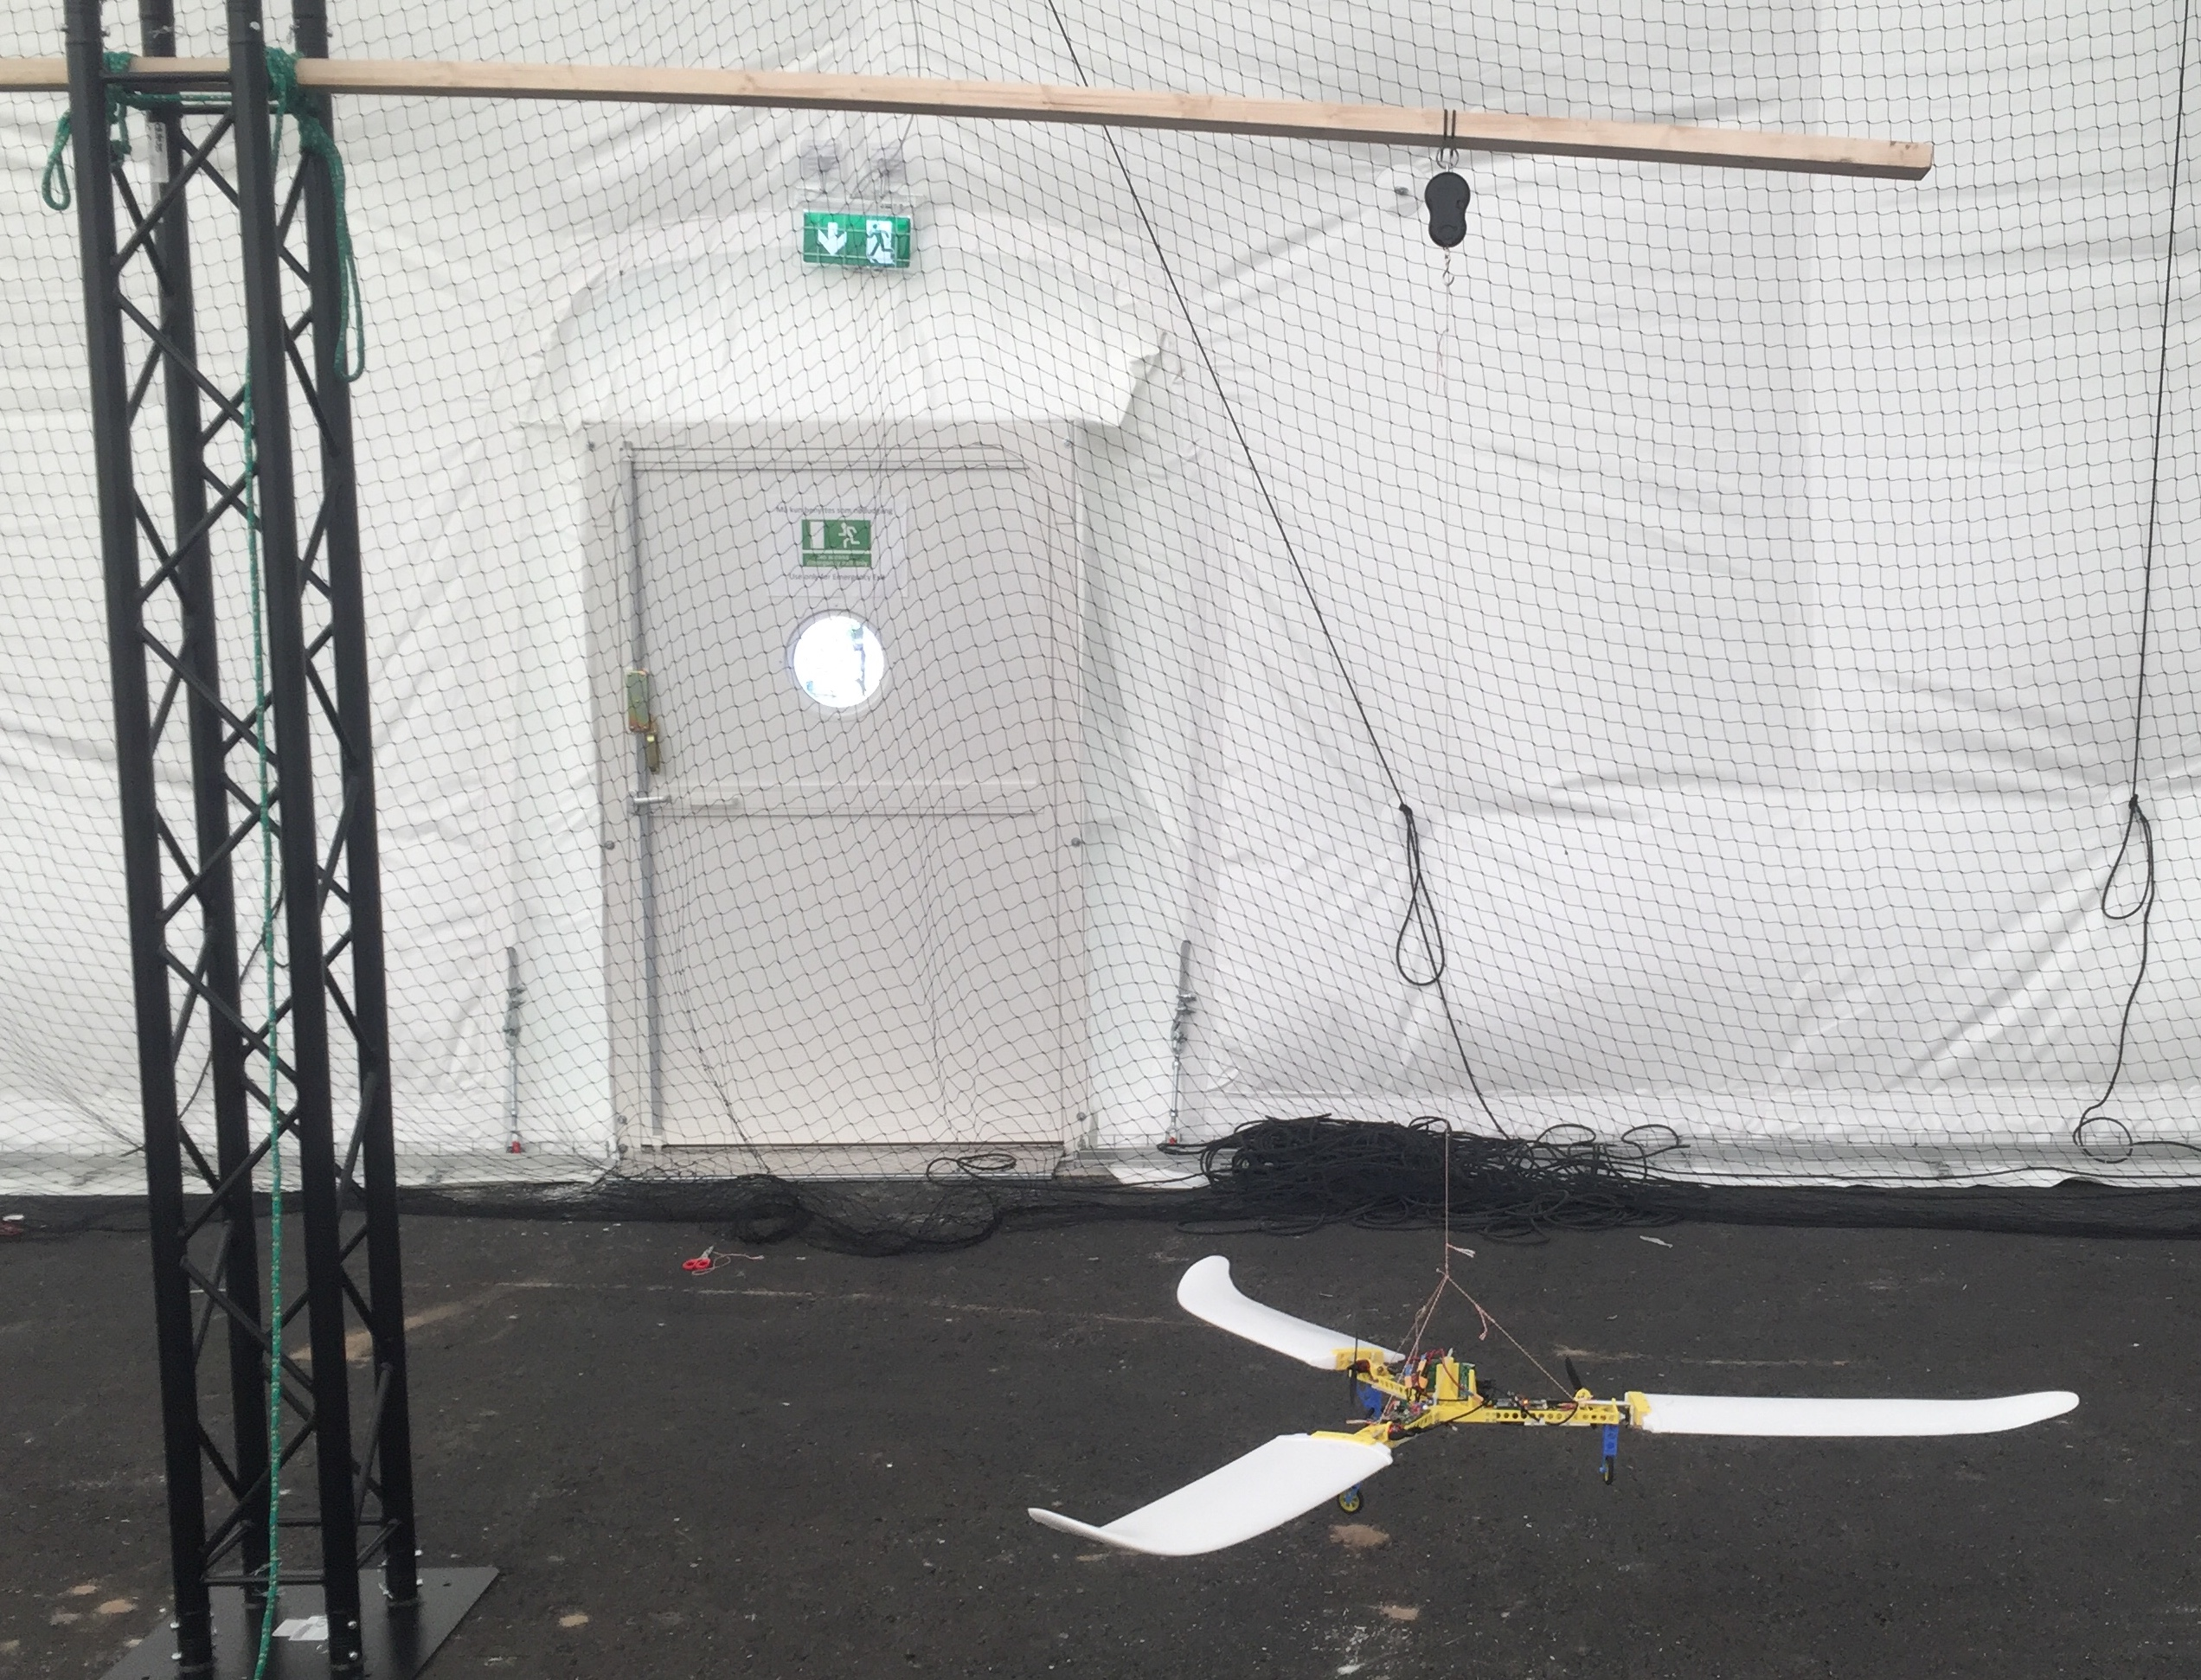
\includegraphics[width=0.7\textwidth]{figures/results/testsetup_air.jpeg}
    \caption{Test setup, air. The drone is hanging from a wooden beam in a cord to simulate in-air behavior}
    \label{fig:testsetup_air}
\end{figure}

\section{Measurement precision}\label{results:measurementprecision}
The precision of the sensor data is crucial for implementing and maintaining reliable controllers on the drone. Thereafter, both the angular velocity and orientation estimations received from the drone are analyzed. 


\subsection{Angular velocity}
The drone's angular velocity sensing is tested by rotating the drone at a constant speed. The rotation is recorded with a video camera and analyzed on a computer. The velocity is tested at PWM of 45\% and 60\% using the ground setup. A comparison of the gathered and recorded data will be made. In this comparison, the measurement of rotational velocity will be converted to rotations per second, because it is challenging to read rotation in radians per second from a video. 

The results of the analysis can be seen in fig. \ref{fig:RPS45PWM} and \ref{fig:RPS60PWM}. 
\begin{figure}[h!]
    \centering
    \begin{minipage}[t]{0.48\textwidth}
        \centering
        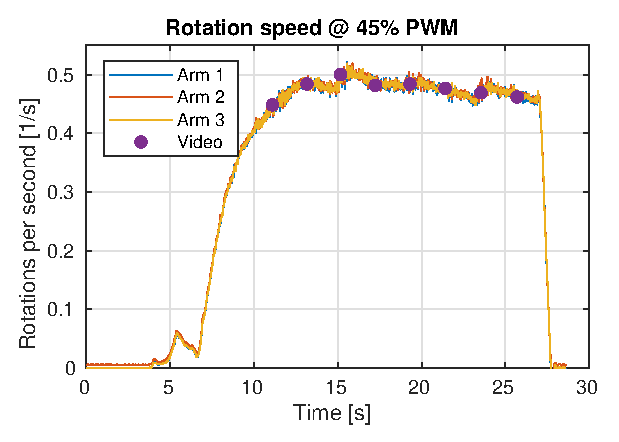
\includegraphics[width=1\textwidth]{figures/results/RPS_45PWM_compared.eps}
    \caption{Rotations per second for PWM at 45\% on ground. Purple dots are from video analysis}
    \label{fig:RPS45PWM}
    \end{minipage}%
    \hspace{.03\textwidth}
    \begin{minipage}[t]{0.48\textwidth}
        \centering
        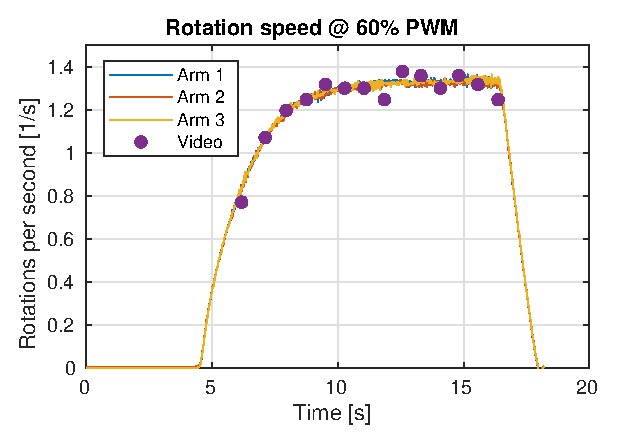
\includegraphics[width=1\textwidth]{figures/results/RPS_60PWM_compared.eps}
    \caption{Rotations per second for PWM at 60\% on ground. Purple dots are from video analysis}
    \label{fig:RPS60PWM}
    \end{minipage}
\end{figure} 
\FloatBarrier
The three lines seen on the figures are each arm's measurement of angular velocity converted to rotations per second. The dots are the rotational speed of the drone derived from the video. Each rotation after the drone started is found and plotted. The start of the recording and start of the drone is lined up as best as possible.


Visually, the distance between points and fits looks very low, especially for PWM at 45\%. The mean square error of the points from the video compared to the sensor data is found to be $MSE_{PWM=45\%} = 6.8220\cdot 10^{-5}$ and $MSE_{PWM=60\%} = 1.8*10^{-3}$. From this it can be concluded, that the measurements of rotational velocity are precise and work as expected.






\subsection{Orientation estimation}
The orientation of the drone is described by roll, pitch, and yaw.  The magnetometer on the drone has been corrected for the local declination of the magnetic field. With the correction, yaw measures the angle from the IMU's x-axis to the true north. 
The ground test-setup was used to examine the drone's ability to estimate its orientation. 
While the drone was rotating, it was recorded from an angle directly above it. This was done for PWM at 40\% and 50\%. 

Continuous measurement of yaw with data from all arms can be seen in fig. \ref{fig:rpm40woodallarms}. 


\begin{figure}[h]
    \centering
    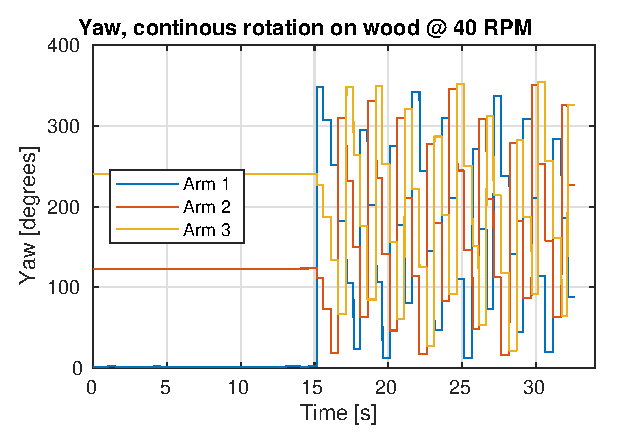
\includegraphics{figures/results/Yaw_rpm40_wood_allarms.eps}
    \caption{Yaw measurements, PWM at 40\% on ground test setup}
    \label{fig:rpm40woodallarms}
\end{figure}
As can be seen, there are about 110 degrees between all arms most of the time. 
The angle doesn't always go all the way to 0 or to 360, but this is also visually exaggerated due to the cyclic nature of angles. Errors related to this will be discussed in section \ref{error_measurementprecision}.


In the analysis of the videos, it was noted each time \texttt{arm 1} had rotated 90 degrees. These points are plotted against \texttt{arm 1's} measurement of the yaw angle. This was done both for RPM at 40\% and 50\% (see fig \ref{fig:rpm40woodvid} and \ref{fig:rpm50woodvid}). 
\begin{figure}[h!]
    \centering
    \begin{minipage}[t]{0.48\textwidth}
        \centering
        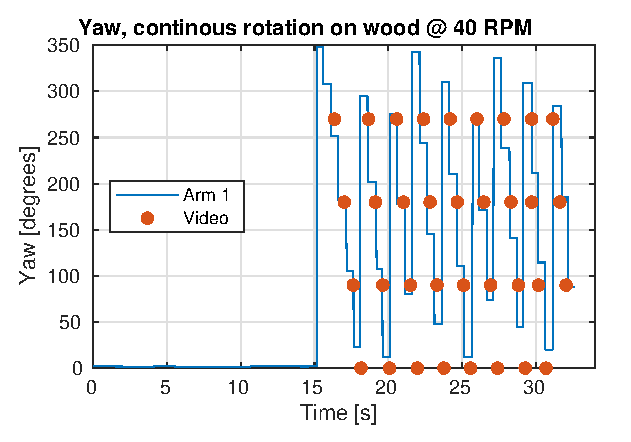
\includegraphics[width=1\textwidth]{figures/results/Yaw_rpm40_wood.eps}
        \caption{Yaw measuremnets, PWM at 40\% on ground test setup, arm 1 and video}
    \label{fig:rpm40woodvid}
    \end{minipage}%
    \hspace{.03\textwidth}
    \begin{minipage}[t]{0.48\textwidth}
        \centering
        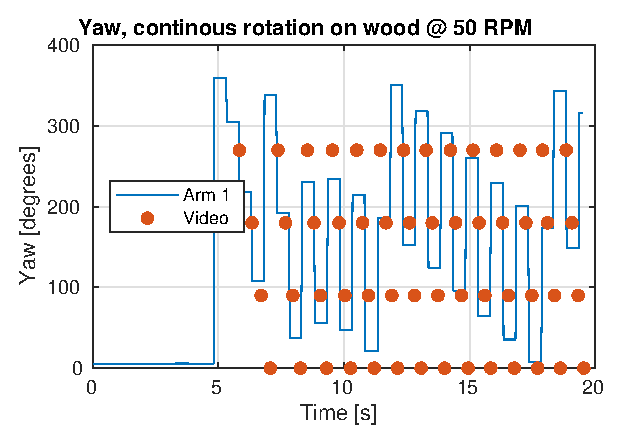
\includegraphics[width=1\textwidth]{figures/results/Yaw_rpm50_wood.eps}
        \caption{Yaw measurements, PWM at 50\% on ground test setup, arm 1 and video}
        \label{fig:rpm50woodvid}
    \end{minipage}
\end{figure} 
Angles of either 0 or 360 degrees from the video analysis, are always plotted as 0 degrees for clarity.
At a PWM of 40 \%, the measured data agree quite well with the video analysis. At higher levels of PWM, the plot starts to lack some data points in the rotation. 

Locating north within $\pm 1$ degrees was never the target goal. A well-calibrated IMU with a Madgwick filter can have a precision of $\pm 4$ degrees \cite{FilterFusionPrecision}. This test shows that it is possible to measure with an accuracy of $\pm 20$ degrees when rotating continuously.  

For the time being, it is somewhat unreliable for higher speeds, but it would be easy to improve (see chapter \ref{sec:communicationimprove}).
Sources of errors and other limitations are discussed in section \ref{error_measurementprecision}.



\subsection{Sources of error} \label{error_measurementprecision}
The general increase in error between video and measured data can be attributed to several things. 
Firstly, due to not having an infinitely high sampling rate on the microcontrollers and its sensors, the error in measurements will naturally increase as the rotational speed increases. 
The sampling rate of the IMU is 100 Hz for the magnetometer, 200 Hz for the gyroscope, and about 1 kHz for the accelerometer. As mentioned previously, the IMU is configured for interrupt-based communication. This limits the update frequency to the lowest common denominator and therefore is 100 Hz. 

Secondly, the video recording was limited to 30 fps. As the picture becomes increasingly blurry, the observer's inability to distinguish angles expectedly grows. The error between the points from the video and the measurements will also increase with velocity. 

Finally, the plots may also make the data look worse than it is. Given that the update frequency only is 30 Hz between RPi and microcontroller, significant data is lost. About 2/3 of all data points are never seen on the RPi, which might explain the lack of "complete rotations" seen in fig. \ref{fig:rpm50woodvid}. At times, the data jumps from 200-300 degrees down to a value slightly above 0 degrees. These jumps are  likely caused by a lack of data on the RPi, rather than lack of data on the microcontroller.

A test of yaw drift can be seen in appendix \ref{fig:yawdrifttest}. It shows no noteworthy drift. 


\section{Wing estimations} \label{chap:wing_est}
The wings' properties were measured with the "in-air" setup. The motors had a constant input voltage, $V_{in} = 3.57 V$ corresponding to a PWM of 30\%. Afterwards, the lift and angular velocity for a varying wing pitch was measured to estimate both the lift and drag coefficients.\\
The lift was measured as a mass with the suitcase-scale on the end of the string carrying the drone. The final lift and angular velocity versus wing pitch can be seen in fig. \ref{fig:lift_omega_measured}.

\begin{figure}[h]
    \centering
    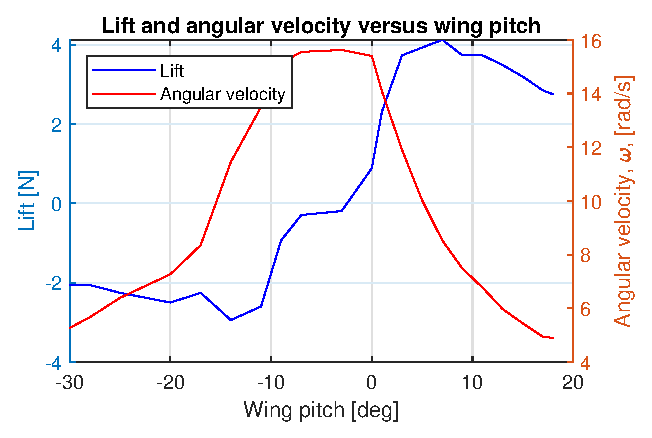
\includegraphics{figures/results/lift_rotation_measured.eps}
    \caption{Lift and angular velocity measured for different wing pitches}
    \label{fig:lift_omega_measured}
\end{figure}

The lift coefficient was estimated from the approach in eq. \ref{eq:cLestimation}. The approach is similar to the one used to calculate the required rotation in eq. \ref{eq:omega_approx}. N is the amount of iterations (here $N=10.000$) and $\Delta R = L_{wing}/N$.
\begin{equation}
\label{eq:cLestimation}
    c_L(\theta) = \frac{1}{3} * \frac{L_{meas}(\theta)*N}{\rho*A_{wing}*\omega^2*\sum_{i=1}^{N} (r_{inner}+ i*\Delta R)^2}
\end{equation}
The comparison of the estimated and measured lift can be seen in fig. \ref{fig:lift_measured}.\\

The drag coefficient at a wing pitch of 0 degrees was adjusted in the Matlab-model until simulations showed similar physical properties to the ones of the drone. This was achieved at a drag coefficient of, $c_{Dbase} = 0.176$ and angular velocity of $\omega_{base} = 15.4 [rad/s]$.\\ 
The subsequent drag coefficients were estimated with eq. \ref{eq:drag_estimation}, since the output power of the motors were the same throughout the test.
\begin{equation}
\label{eq:drag_estimation}
    c_D(\theta) = \left(\frac{\omega_{base}}{\omega_{\theta}}\right)^2* c_{dBase}
\end{equation}
The resulting drag coefficients can be seen compared to the Foil Sim Applet's estimation in fig. \ref{fig:drag_measured}. Furthermore, measured lift coefficients compared to Foil Sim Applet's estimation can be seen in fig \ref{fig:lift_measured}.\\
Both the drag and lift coefficients measured deviate significantly from the ones obtained from the applet. This can be partially explained by the imprecise scale (meant for weighing suitcases) and the fact that the drone does oscillate slightly away from directly underneath the string. These results are prone to many errors caused by a series of underlying approximations and assumptions. The complexity of aerodynamics shall not be underestimated; however, these results work decently for testing purposes.

\begin{figure}[h!]
    \centering
    \begin{minipage}[t]{0.48\textwidth}
        \centering
        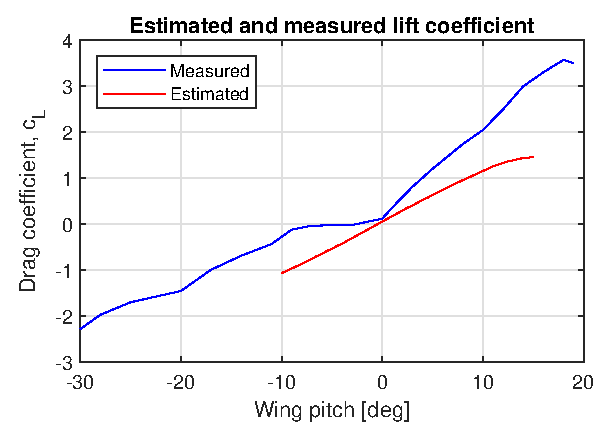
\includegraphics[width=1\textwidth]{figures/results/lift_measured.eps}
    \caption{Lift coefficient measured with the test rig compared to the estimated lift coefficient from the Foil Sim Applet}
    \label{fig:lift_measured}
        
    \end{minipage}%
    \hspace{.03\textwidth}
    \begin{minipage}[t]{0.48\textwidth}
        \centering
        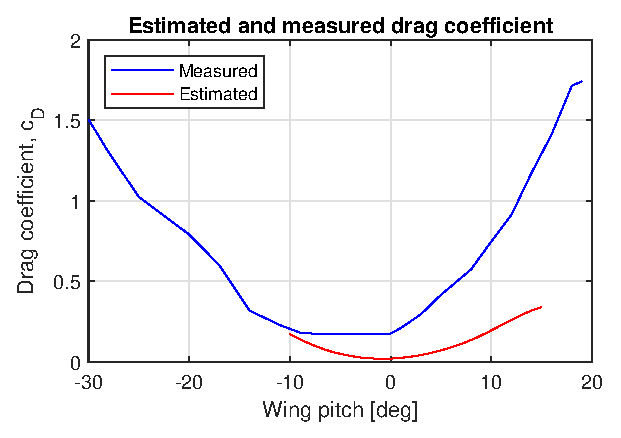
\includegraphics[width=1\textwidth]{figures/results/drag_measured.eps}
    \caption{Drag coefficient measure estimation with the test rig compared to the coefficients from the Foil Sim Applet}
    \label{fig:drag_measured}
    \end{minipage}
\end{figure} 
Fig. \ref{fig:LDratio_measured} is a plot of the lift-to-drag ratio measurement and Foil Sim estimation.
\begin{figure}[h]
    \centering
    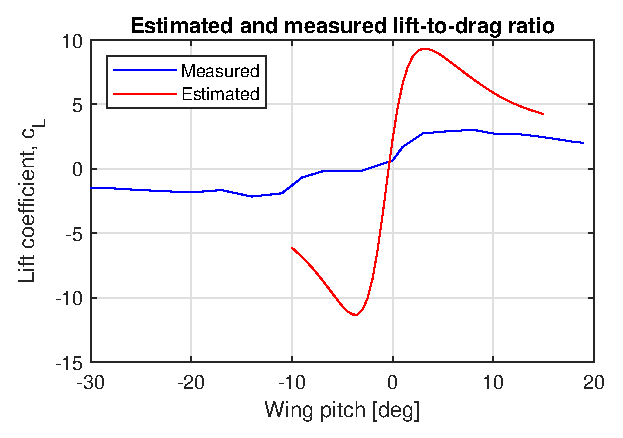
\includegraphics{figures/results/LDratio_measured.eps}
    \caption{Lift-to-drag ratio as measured and estimated with the Foil Sim Applet}
    \label{fig:LDratio_measured}
\end{figure}
\newpage

\section{Rotation controller and system response}\label{results:rotcontroller}
Transfer functions will be derived for the system in three different states and one for the model. First state is a grounded system. Second state is in the air with minimal drag. Third state is in the air with some drag. The functions will be analyzed and compared to each other, to examine the difference between states as well as model compared to the real world. 
Eventually the final controller will be derived and implemented. 


\subsection{Deriving transfer functions}
To derive a transfer function, the theory in section \ref{tf_teori} is used. The system received a step of PWM from 35\% to 39\%, and is analysed both on the ground and in the air. This value interval might seem arbitrary, but was chosen, as it is high enough to let the drone rotate both on the ground and in the air, yet low enough so the drone is easily observable. Furthermore, in the air, it is stepped both with minimal drag and some drag. This was chosen to investigate if there was any notable difference between the system responses in the three cases. 
% When using System Identification Toolbox, a guess of a system with 1 pole and 2 poles are made. This is due to having a low sampling frequency, so time constants from the motors and other really fast components are not visible. One constant is expected from the inertia of the drone due to its size, and one for 

\subsubsection{Grounded system}
The step from PWM of 35 \% to 39\% is made using the ground test-setup and can be seen in fig. \ref{fig:stepwood}.
\begin{figure}[h!]
    \centering
    \begin{minipage}[t]{0.48\textwidth}
        \centering
        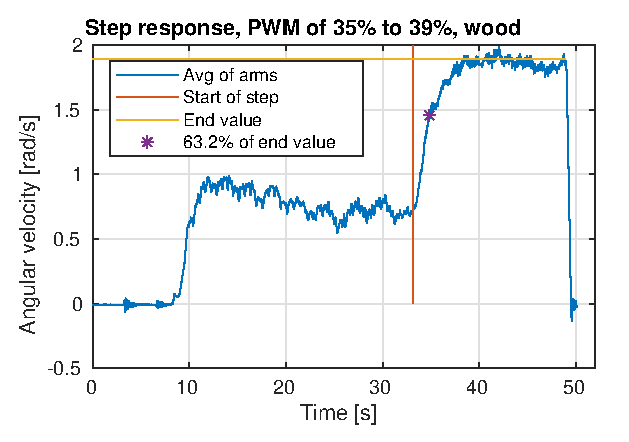
\includegraphics[width=1\textwidth]{figures/results/stepwood.eps}
        \caption{Step on wooden surface using the ground test-setup}
        \label{fig:stepwood}
    \end{minipage}%
    \hspace{.03\textwidth}
    \begin{minipage}[t]{0.48\textwidth}
        \centering
        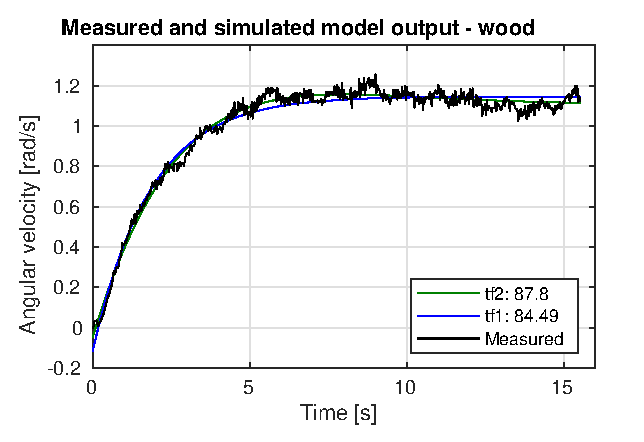
\includegraphics[width=1\textwidth]{figures/results/stepwood_sysid.eps}
        \caption{Plot from System Identification Toolbox. $Tf_1$ is 1 pole, $Tf_2$ is two poles. The data was offset to start in 0}
        \label{fig:stepwoodsysid}
    \end{minipage}
\end{figure} 
This looks quite similar to a 1st or 2nd order system. One might expect a system with more poles, but with the low sampling frequency smaller time constants (e.g. electrical) cannot be measured. \\
Assuming a 1st order system and analysing the step, the time constant is found as $\tau_1 = 1.6404$. The pole is $p_1 = -0.6096$. \textit{b} can then be calculated:

\begin{equation}
    b = \frac{y_{final} - y_{init}}{x_{final}}* a =  \frac{1.89-0.71}{4.5} \cdot 0.6096 = 0.1603
\end{equation}

The manually derived transfer function becomes:
\begin{equation}\label{eq:woodsysman}
    tf_{manual} = \frac{0.1603}{s+0.6096}
\end{equation}

Analysing the step with System Identification Toolbox, the following step and transfer functions are derived, see fig. \ref{fig:stepwoodsysid} as well as eq. \ref{eq:woodsysid1} and \ref{eq:woodsysid2}. 


\begin{equation}\label{eq:woodsysid1}
    tf_1 = \frac{0.1387}{s+0.5383}
\end{equation}
\begin{equation}\label{eq:woodsysid2}
    tf_2 = \frac{0.03641}{s^2 + 0.6571 s + 0.1462}
\end{equation}
The transfer function found manually in eq. \ref{eq:woodsysman} and the two found with System Identification Toolbox, are very similar. The two 1st order systems have poles in approximately the same places and almost the same gain. 
The 2nd order system has a complex pole pair located at $-3.29 \pm 0.196 I$. The complex poles are presumably caused by either flex in the wheel mounting, or due to the vibration introduced from the wooden surface. 






\subsubsection{Airborne system with minimal drag}\label{sec:airminimal}
The step of the system was made with the air test-setup, see fig. \ref{fig:steprope}.
\begin{figure}[h!]
    \centering
    \begin{minipage}[t]{0.48\textwidth}
        \centering
        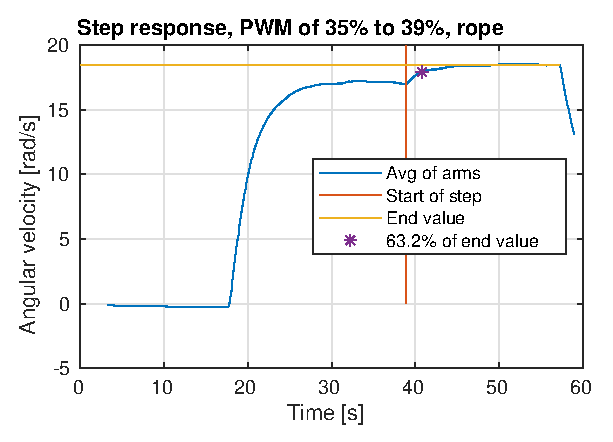
\includegraphics[width=1\textwidth]{figures/results/steprope.eps}
        \caption{Step using air test-setup}
        \label{fig:steprope}
    \end{minipage}%
    \hspace{.03\textwidth}
    \begin{minipage}[t]{0.48\textwidth}
        \centering
        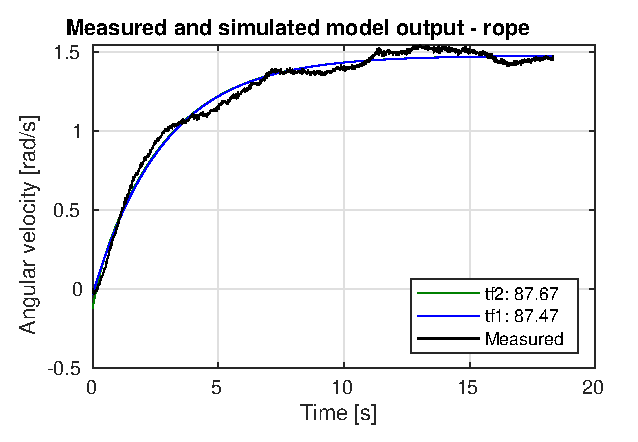
\includegraphics[width=1\textwidth]{figures/results/steprope_sysid.eps}
        \caption{Plot from System Identification Toolbox, $Tf_1$ is 1 pole, $Tf_2$ is 2 poles. The data was offset to start in 0}
        \label{fig:stepropesysid}
    \end{minipage}
\end{figure} 

Analyzing the step with System Identification Toolbox, the fits can be seen in fig. \ref{fig:stepropesysid}, and transfer functions in eq. \ref{eq:airsysid1} and \ref{eq:airsysid2}.

\begin{equation}\label{eq:airsysid1}
    Tf_1 = \frac{0.1132}{s+0.3523}
\end{equation}
\begin{equation}\label{eq:airsysid2}
    Tf_2 = \frac{0.4608}{s^2 + 4.439s+1.434}
\end{equation}
The first pole for the 1st order and 2nd order system is practically identical at respectively $-0.3523$ and $-0.3507$. Due to its very low frequency, this pole probably correlates to the inertia of the drone. \\
The second pole for the 2nd order system is at $-4.088$, and corresponds to a very small time constant. The second, less dominant, pole might possibly be the pole associated with the mechanical time constant of the motors \cite{motordata} (see also section \ref{sec:modelresponse}) .

\subsubsection{Airborne system with more drag}
The step was made using the air test-setup, but this time with a 5 degrees tilt of the wings (positive angles creates lift). The step response can be seen fig. \ref{fig:steprope65}.

\begin{figure}[h!]
    \centering
    \begin{minipage}[t]{0.48\textwidth}
        \centering
        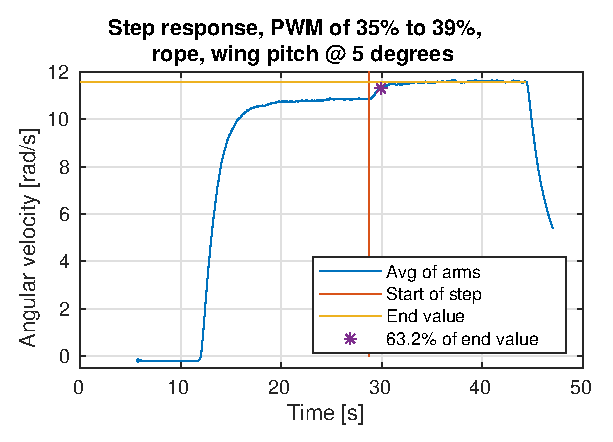
\includegraphics[width=1\textwidth]{figures/results/steprope65degrees.eps}
        \caption{Step using air test-setup with a pitch angle of $\sim$5 degrees}
        \label{fig:steprope65}
    \end{minipage}%
    \hspace{.03\textwidth}
    \begin{minipage}[t]{0.48\textwidth}
        \centering
        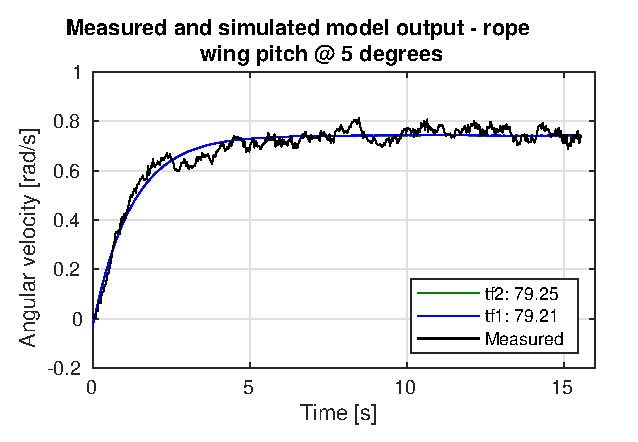
\includegraphics[width=1\textwidth]{figures/results/steprope65degrees_sysid.eps}
        \caption{Plot from System Identification Toolbox, $Tf_1$ is 1 pole, $Tf_2$ is 2 poles. The data was offset to start in 0. Pitch angle was $\sim$5 degrees}
        \label{fig:steprope65sysid}
    \end{minipage}
\end{figure} 

With System Identification Toolbox, the following fits and transfer functions are found, see fig. \ref{fig:steprope65sysid} as well as eq. \ref{eq:air65sysid1} and \ref{eq:air65sysid2}. 


\begin{equation}\label{eq:air65sysid1}
    Tf_1 = \frac{0.1311}{s+0.8044}
\end{equation}
\begin{equation}\label{eq:air65sysid2}
    Tf_2 = \frac{3.862}{s^2 + 29.91s + 23.7}
\end{equation}
The 2nd order system's poles are real and located at $p_1=-0.815$ and $p_2=-29.095$. The first pole from the 2nd order system is very close to the pole from the 1st order system. This second pole is much smaller than the second pole for the case with minimal drag. This clearly outlines some nonlinear component in the system and may very well be caused by the drag. 


\subsubsection{Comparison of systems}
The systems on wheels and in the air are very similar in terms of time constants, but the resistance from rolling associated with the wheels create a large offset. With a PWM of 35\%, the angular velocity in the air is about 16 rad/s, but on the ground, it is approximately 0.8 rad/s. This is a massive loss in rotational energy. Furthermore, the absolute increase in amplitude for the steps on the ground and in the air is about the same, which means the rolling resistance does not increase appreciably with angular velocity. \\ 
The dominating time constant for the case with some drag is faster than the one with minimal drag, but the system also reaches a far lower amplitude. The minimal drag case's relative increase in amplitude is 1.5 but is only 0.75 for the case with some drag. Due to non-linear components, there is a notable difference between the two step-responses, both in terms of steady-state error and pole placement. This can be solved with gain scheduling, though this concept will not be explored further in this thesis. 


\subsection{Modelled system's response}\label{sec:modelresponse}
The model transfer function was derived in a similar fashion to the method above. At a steady state rotation the input voltage of $V_{in} = 0.35*11.9V = 4.17 \,V$ was stepped to $V_{in} = 0.39*11.9V = 4.641\,$. The model's step response was analyzed with the help of the Tfest-function in the System Identification's Toolbox (fig. \ref{fig:bode_tfest}). The steady state gain was measured to 0.9 for the Simulink model.
\begin{figure}[h]
    \centering
    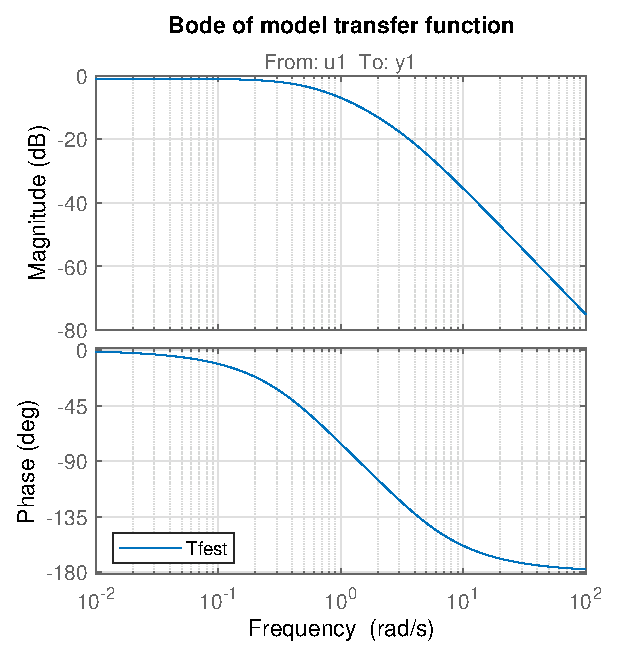
\includegraphics{figures/results/bode_tfest.eps}
    \caption{Bode plot of model's transfer function; voltage to angular velocity}
    \label{fig:bode_tfest}
\end{figure}
The system approximated with Tfest is a 2nd order continuous system, with a fit of 99.4\%. The transfer function for this system is: 
\begin{equation}
    M(s) = \frac{1.77}{s^2+3.82*s+1.96}   
\end{equation}
The poles for this transfer function are $p_1 = -0.61$ and $p_2 = -3.21$. \\
Similarly, by measuring the time constants "by hand" for the drone's angular velocity, $\omega$ and the motors' RPM in the model, the poles become: $p_{\tau \omega} = -0.535$ and $p_{\tau RPM} = -6.87$.  \\
By comparing these two sets of poles, with the transfer function derived in section \ref{sec:airminimal}, it's seen that the modelled system is indeed a good approximation of the real drone. Each pole is roughly within a factor of two of its equivalent pole. Furthermore, it supports the theory that the two lowest frequency poles of the system are associated with the inertia of the system and the mechanical pole in the prop motor.


\subsection{Final controller and implementation}
\subsubsection{Feed-forward gain estimation}
The feed-forward branch was determined by inputting different voltages and recording the drone's steady-state angular velocity. The fit and plot of these data can be seen in fig. \ref{fig:kfestimation}.
\begin{figure}[h!]
    \centering
    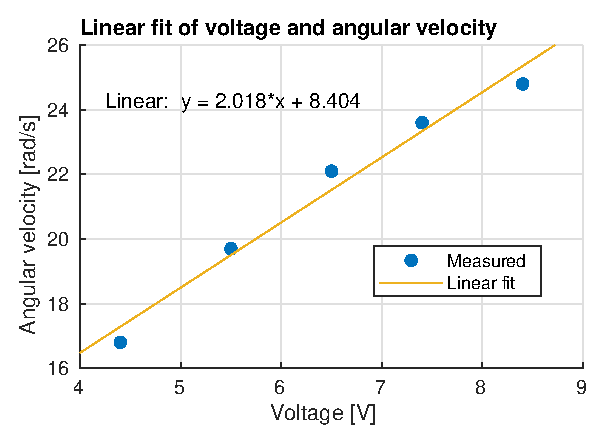
\includegraphics{figures/results/feedforwardfit.eps}
    \caption{Linear fit of angular velocity versus input voltage}
    \label{fig:kfestimation}
\end{figure}
The angular velocity versus input voltage can be approximated as a linear relationship. The gain from the reference $\omega$ to the summation node (see also fig. \ref{fig:controlblock}) before the system becomes:
\begin{equation}
    V = -4.16 + 0.50*\omega_{ref}
\end{equation}
The constant offset is because the motor will not turn on below an input PWM of 13\%.\\

\subsubsection{Proportional and differential gain}
Since the rough input voltage to the system is taken care of by the feed-forward branch, the $K_p$ does not need to be very large. The $K_p$ was found to generate stable results on the model within the ranges of $K_p = [0.7;1.5]$.\\
Equally, the differential gain, $K_d$, needed to be large enough to dampen any unnecessarily large accelerations, but not so large that the response time was too long. For the implementation, the derivative gain was finalized at $K_d = 0.9$. This dampens the oscillations sufficiently.\\
The final implemented controller (including the feed-forward branch) is as seen in eq. \ref{eq:finalcontroller}; $e(t)$ is the time dependent error.
\begin{equation}
    \label{eq:finalcontroller}
    V(t) = 1.3 + 0.9*\frac{de(t)}{dt}+(\omega_{ref}*0.50-4.16)
\end{equation}
The complete system is stable with an infinite phase margin. However, there is a steady-state error of -2.6 dB; see fig. \ref{fig:systemcontrollerbode}. The derived system with the pitched wing is stable with this controller but will experience a larger steady-state error (fig. \ref{fig:systempitchcontrollerbode}). This is because of the generally non-linear behavior of the velocity. The consequence will be, that the controller will not be a one-size-fits-all solution, but rather a compromise of being stable and precise around the operating point of $\theta_{wing} = 0 \,deg$. \\

\subsubsection{Step response with controller}
The drone was tested with the controller using the air setup. It started from an initial velocity of 0 and a reference point of $\omega_{ref} = 15 \, \text{rad/}$. When the drone had reached steady state, its reference point was changed to $\omega_{ref} = 20 \, \text{rad/s}$. The sensor measurements of the step can be seen in fig. \ref{fig:stepwithcontroller}.
\begin{figure}[h]
    \centering
    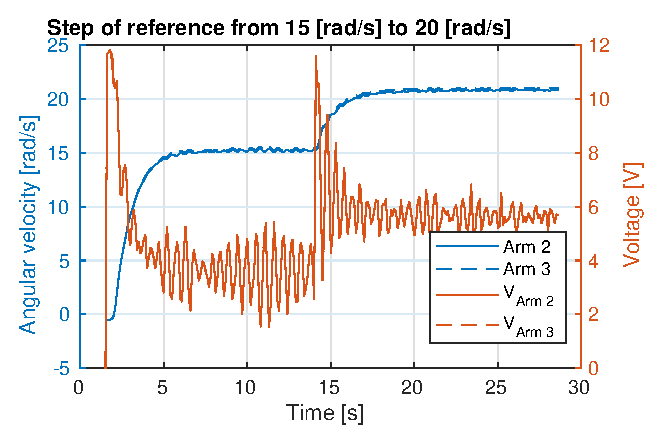
\includegraphics{figures/results/stepwithcontroller.eps}
    \caption{Closed-loop step with controller. From $\omega_{ref} = 15\, \text{rad/s}$ to $\omega_{ref} = 20\, \text{rad/s}$}
    \label{fig:stepwithcontroller}
\end{figure}
For the initial reference point the drone settles at an angular velocity of $\omega_{out} = 15.27 \,\text{rad/s}$.

\begin{table}[h]
\centering
\resizebox{0.5\textwidth}{!}{%
\begin{tabular}{|l|l|}
\hline
Time domain specification & Value \\ \hline
Rise time                 & 2.4 [s] \\ \hline
Settling time             & 9.3 [s] \\ \hline
Peak time                 & 12.1 [s] \\ \hline
Overshoot                 & 4.95 \%     \\ \hline
Steady state error        & $0.92\, [\text{rad}/\text{s}]$ \\ \hline
\end{tabular}%
}
\caption{Time domain specifications for system with controller and feed-forward}
\label{tab:timedomainspecs_step}
\end{table}
For both reference points, the controlled system experiences a steady-state error as one might expect from inspecting the closed-loop frequency response. However, this steady-state error is much smaller than what the closed-loop frequency response indicates.\\
This could be the result of the somewhat low sensor sampling rate of about $f_{s} = 100 \,\text{Hz}$. Some poles related to the constants of the motor are likely to be at much higher frequencies.\\
Furthermore, this steady-state error is a necessary compromise for the system. The proportional gain is limited to small values because the motor voltage is confined to values between 0 and the battery voltage. Thus, this rather small steady-state error is a beneficiary compromise of the stable system. \\
In table \ref{tab:timedomainspecs_step}, the step time domain specifications of the system with controller and feed-forward are listed. The final controlled system is considerably fast with a 2.4s rise time; however, this does introduce some overshoot.\\

Additionally, one of the sensors stopped working for the drone's final testing with the controller, leading to less accurate measurements, which does play a role in the error that the controller uses.



\section{Flying the drone}\label{chap:flydrone}
Finally, the drone is not complete without a proper test flight. The test flight was done while attached to the "in-air" setup. The flight procedure was done without the rotational controller. \\
The procedure for "flying" was:
\begin{enumerate}
    \item Accelerate drone to an obtainable speed at 80\% of the maximal voltage with 0 degree wing pitch
    \item Set the wing pitch to roughly 10 degrees upwards.
\end{enumerate}
\begin{figure}[h]
    \centering
    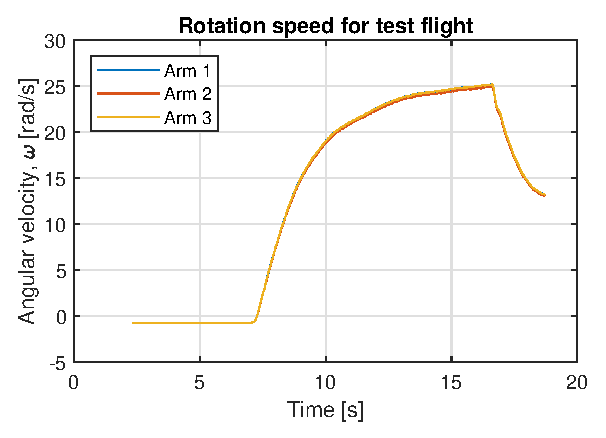
\includegraphics{figures/results/flight_rotational_velocity.eps}
    \caption{Rotational velocity of the drone for flight tests. At $\sim$16.5 seconds, the pitch angle was changed to generate lift}
    \label{fig:rotationflight}
\end{figure}
This procedure did not result in continuous flight but did create a burst of enough lift such that the drone changed its z-position by around $0.5$m above its initial position. Afterwards, it slowly soared down to the original height as all its built-up kinetic energy had been transferred into mechanical lift and drag.\\
Since the motors were only throttled to 80\% of their maximum, they could indeed have been able to sustain a hover condition. However, at very high speeds, the drone loses stability about its horizontal axis and starts swinging heavily from side to side.\\
The rotational velocity seen in fig. \ref{fig:rotationflight} is well above the required rotation for hover with a wing pitch of 10 degrees (fig. \ref{fig:lift_measured}).
A link to a video of the "flight" can be found in appendix \ref{link:droneflight}. 



\section{Power use} \label{sec:poweruse}
With regards to power usage, there are especially two things to be consider when estimating usage. First the prop motors draw a rather large current when running, so any loss within the wires and PCB can be neglected. Secondly, the input current to each PCB can be assumed equal to the input current to the motors. The voltage-power relationship can be seen in fig. \ref{fig:power} (with a wing pitch of $\theta_{wing} = 0 \,deg$). Comparing this angular velocity with the ones calculated in fig. \ref{fig:liftvariation} and the measured lift in fig. \ref{fig:lift_omega_measured}, it is seen that a slight pitch of the wing would indeed slow the drone's rotation, but create the lift necessary to hover. This means that this power output is a decent estimate of the one required in a hover state.\\
\begin{figure}[h!]
    \centering
    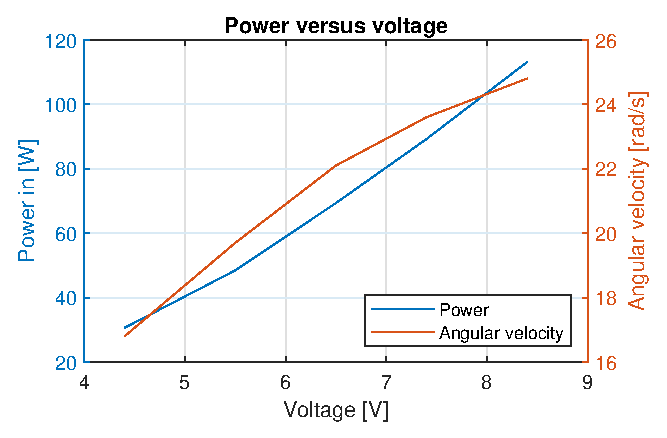
\includegraphics{figures/results/power_voltage.eps}
    \caption{Input power of all prop motors versus voltage; includes recorded angular velocity}
    \label{fig:power}
\end{figure}
The power draw is quite low compared to drones like the one mentioned in section \ref{sec:stateoftheart}, but the battery in use is also small. This means, that with the current setup the flight time will not be very long. How to increase the duration will be discussed in section \ref{sec:futureworkphysicalchanges}. 




\section{Chapter summary}
The sensor measurements were tested and found to be successful. Additionally the sensor fusion algorithm was tested. It was seen that the internal sampling rate of the compass in the IMU had a restricting effect on the algorithm's accuracy. The wing approximation was tested with the real drone's behavior at different AoA. The drone's natural transfer function was also derived both on and off ground for further analysis. Furthermore the model's transfer function was derived. The drone's controller was analysed and implemented with success. It was also shown that the drone is able to fly under the right conditions. All objectives outlined in section \ref{sec:objectives} and \ref{analysisofgoals} were achieved. 